Kontekst ten pełni funkcję głównego mechanizmu budowania specyfikacji produktowej oraz walidacji technologicznej. Oddziela on złożone drzewo reguł (wykluczeń i wymagań technologicznych narzuconych przez producenta) od samego faktu zawarcia transakcji, która procesowana jest w niezależnym module Sprzedaży.

\subsubsection{Kanwa Kontekstu Katalogu i konfiguratora}

\begin{figure}[H]
    \centering
    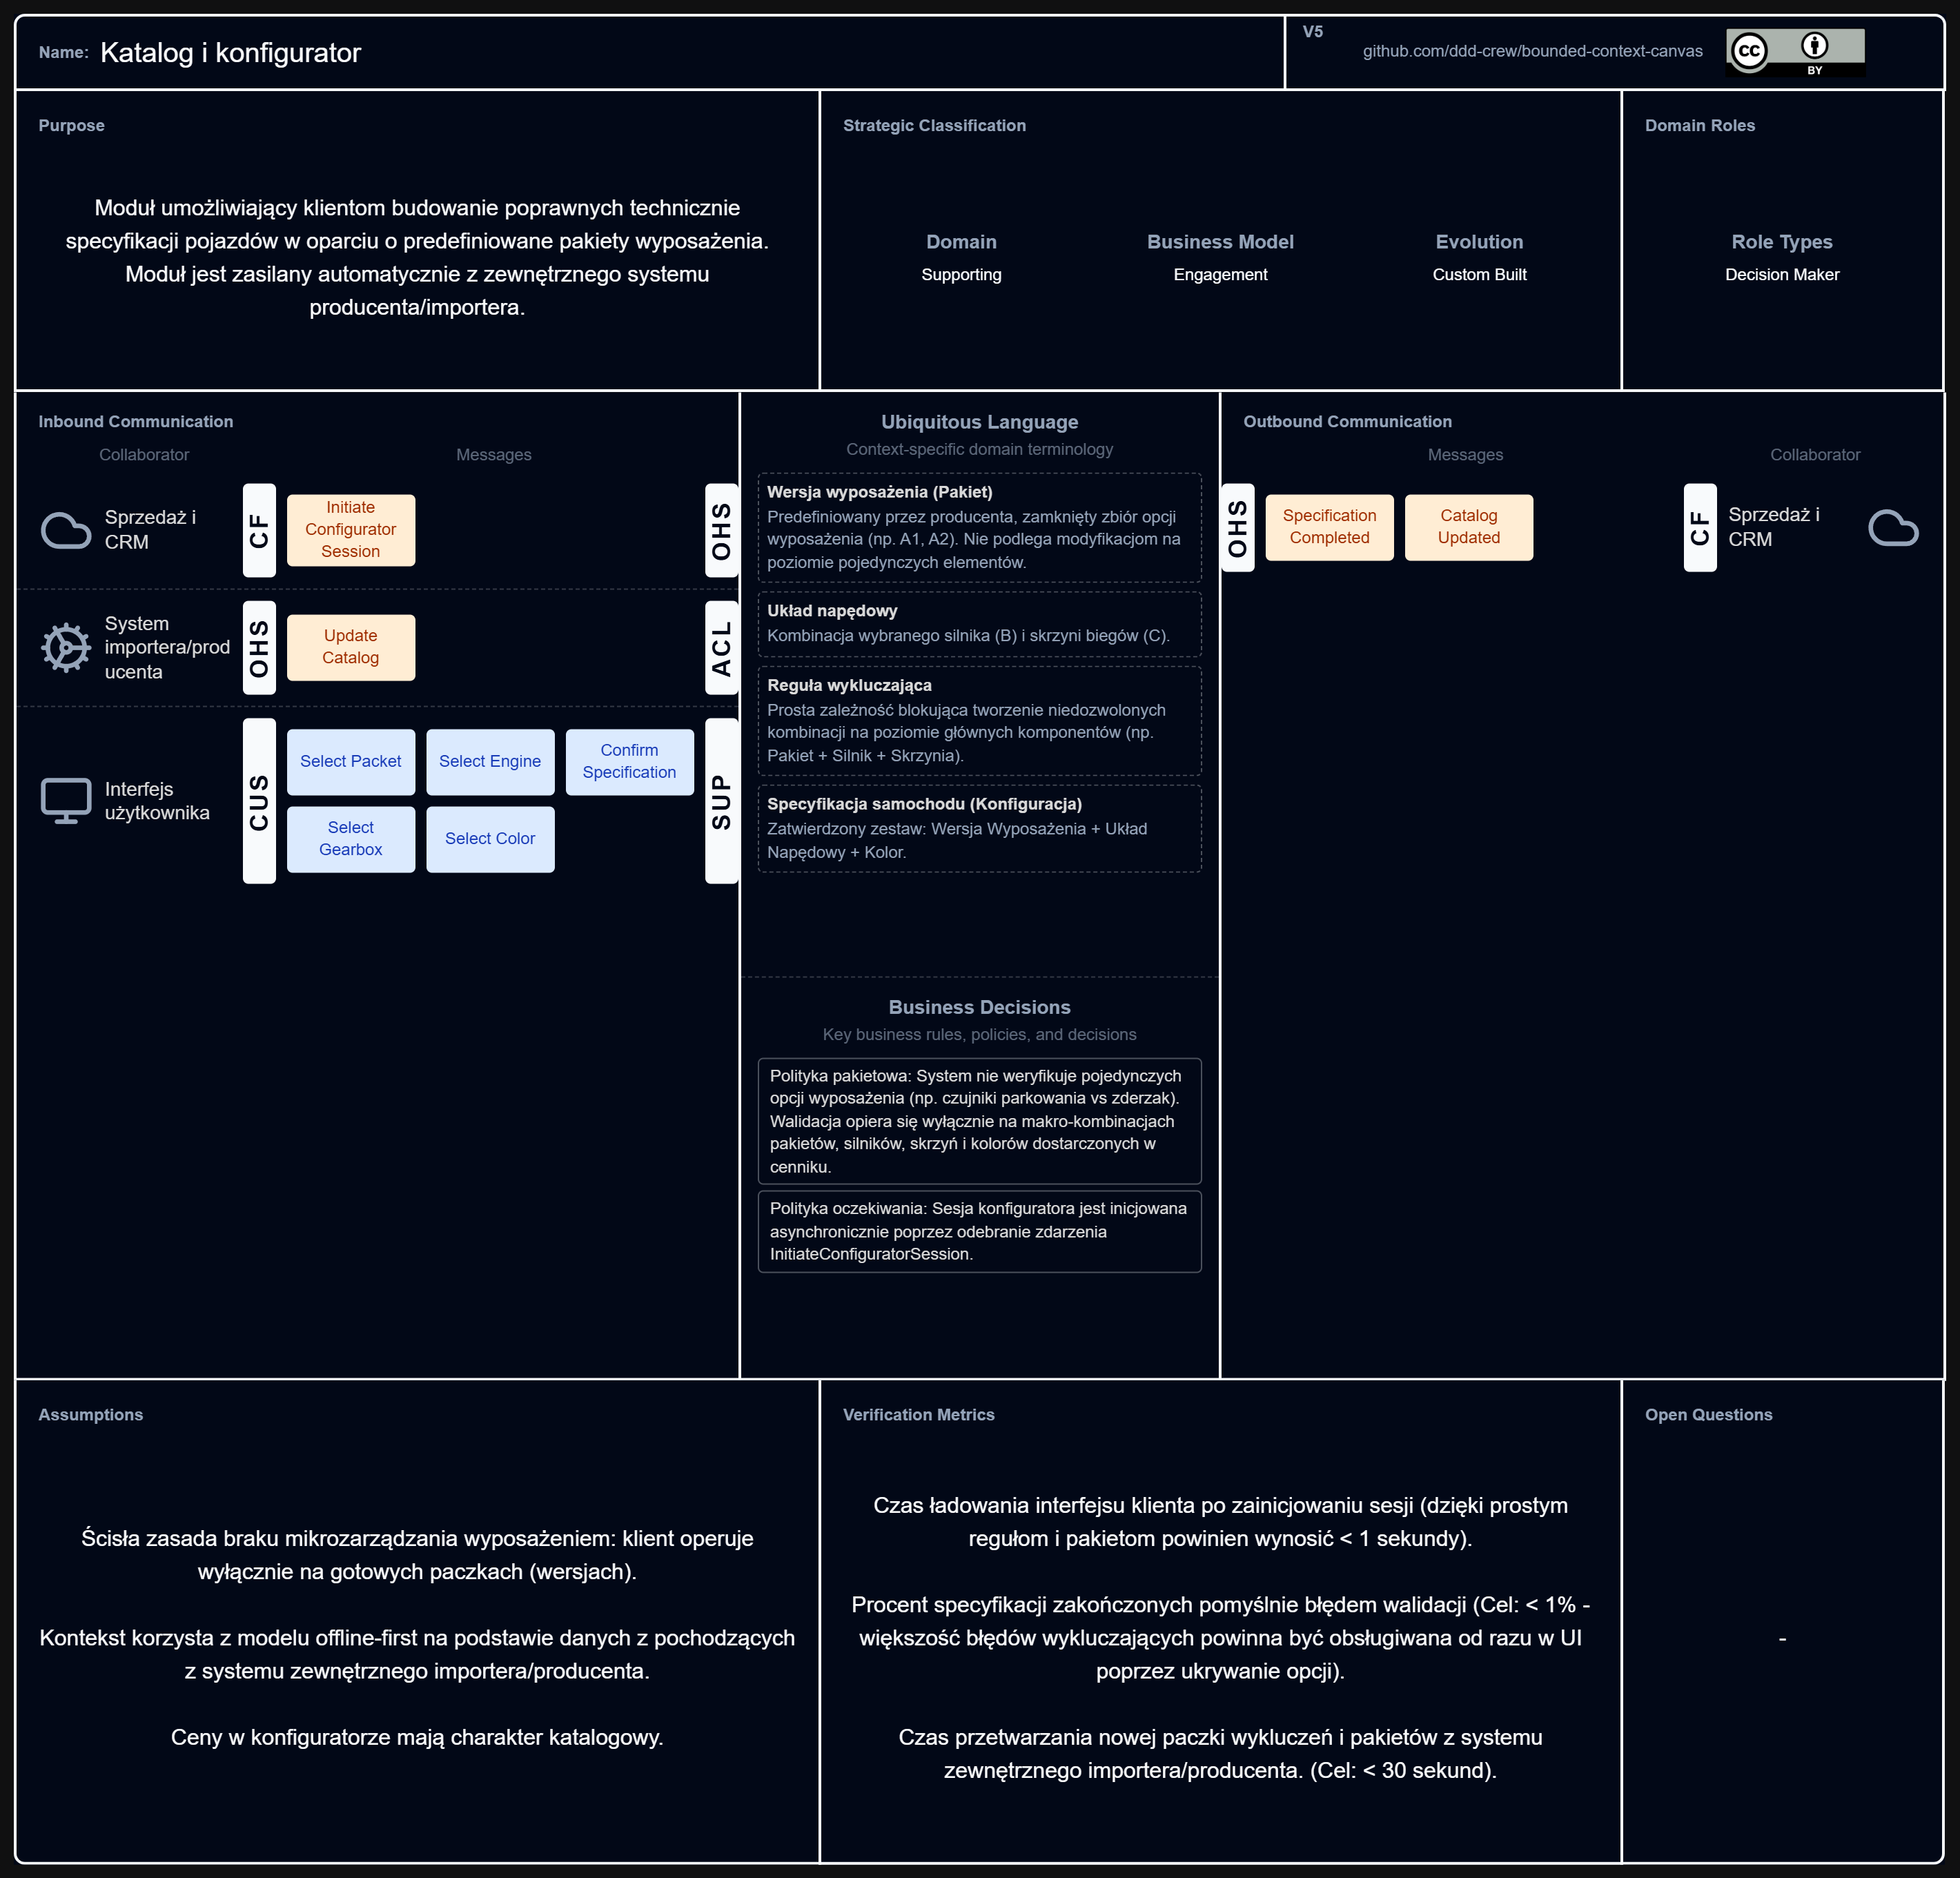
\includegraphics[width=\textwidth]{media/bounded-context-canvas/final/KIK_K2_TOTAL_FINAL.png}
    \caption{Kanwa Kontekstu  Katalogu i konfiguratora}
    \label{fig:hex_billing}
\end{figure}


\subsubsection{Przypadki użycia Kontekstu Katalogu i konfiguratora}
% =====================================================
\textbf{UC-KON-01: Opracowanie i zatwierdzenie specyfikacji pojazdu}

\begin{longtable}{|p{4cm}|p{11cm}|}
\hline
\textbf{Element} & \textbf{Opis} \\
\hline

Identyfikator & UC-KON-01 \\
\hline

Nazwa & Opracowanie i zatwierdzenie specyfikacji pojazdu \\
\hline

Opis & 
Proces wyboru parametrów pojazdu oparty na predefiniowanych pakietach wyposażenia, silnikach, skrzyniach biegów oraz kolorach nadwozia, zakończony zatwierdzeniem konfiguracji. \\
\hline

Aktor główny & Klient \\
\hline

Aktorzy pomocniczy & -  \\
\hline

Warunki wstępne & 
Kontekst Katalog i Konfigurator otrzymał zdarzenie \textit{InitiateConfiguratorSession}. \\
\hline

Warunki końcowe & 
Zatwierdzona specyfikacja zostaje zapisana w lokalnej bazie danych konfiguratora, a system emituje zdarzenie \textit{SpecificationCompleted}. \\
\hline

Scenariusz główny & 
\begin{enumerate}
    \item System otwiera sesję konfiguratora i prezentuje Klientowi interfejs z modelami samochodów, wersjami wyposażenia (np. pakiet A1, A2), silnikami (np. B1, B2), rodzajami skrzyni biegów (np. C1, C2) oraz kolorami.
    \item Klient wybiera jeden główny pakiet wyposażenia (np. A1).
    \item Klient dobiera do pakietu silnik (np. B1), rodzaj skrzyni biegów (np. C1) oraz kolor.
    \item System na bieżąco weryfikuje proste reguły wykluczające (np. silnik B2 nie może być wybrany ze skrzynią biegów C1).
    \item Klient zatwierdza specyfikację.
    \item System weryfikuje ostateczną kompletność konfiguracji.
    \item System zapisuje specyfikację i emituje zdarzenie \textit{SpecificationCompleted}.
\end{enumerate} \\
\hline

Scenariusze alternatywne & 
\begin{itemize}
    \item [A1] Niedozwolona kombinacja: W kroku 4 system wykrywa, że wybrana kombinacja jest zablokowana przez producenta (np. silnik B2 nie może być wybrany ze skrzynią C1). System blokuje możliwość zatwierdzenia i prosi Klienta o zmianę silnika, skrzyni biegów lub pakietu. Kontekst nie emituje zdarzenia końcowego.
    \item [A2] Przerwanie sesji: Klient opuszcza konfigurator przed zatwierdzeniem. System zapisuje konfigurację jako wersję roboczą.
\end{itemize} \\
\hline
\end{longtable}

\begin{figure}[H]
    \centering
    \includegraphics[width=1\textwidth]{media/diagramy_sekwencji/kontekst-katalog/UC-KON-01-Sekwencji.png}
    \caption{Diagram sekwencji dla przypadku użycia UC-KON-01: Opracowanie i zatwierdzenie specyfikacji pojazdu}
    \label{fig:seq_uc_kon_01}
\end{figure}

% =====================================================
\textbf{UC-KON-02: Automatyczna aktualizacja cennika i katalogu}

\begin{longtable}{|p{4cm}|p{11cm}|}
\hline
\textbf{Element} & \textbf{Opis} \\
\hline

Identyfikator & UC-KON-02 \\
\hline

Nazwa & Automatyczna aktualizacja cennika i katalogu \\
\hline

Opis & 
Zautomatyzowany proces pobierania, walidacji i zapisu nowego katalogu modeli oraz cennika, inicjowany przez zewnętrzny system producenta/importera (Blackbox). \\
\hline

Aktor główny & Zewnętrzny system producenta/importera \\
\hline

Aktorzy pomocniczy & - \\
\hline

Warunki wstępne & 
System zewnętrzny importera/producenta udostępnia nowy pakiet danych katalogowych (np. poprzez webhook, szynę zdarzeń lub API). \\
\hline

Warunki końcowe & 
Lokalna baza konfiguratora zostaje zaktualizowana, a kontekst emituje zdarzenie \textit{CatalogUpdated}. \\
\hline

Scenariusz główny & 
\begin{enumerate}
    \item Kontekst odbiera sygnał/dane o nowym cenniku z systemu Blackbox (np. poprzez zdarzenie integracyjne lub żądanie API).
    \item System parsuje otrzymany pakiet danych, wykorzystując warstwę translacji (ACL), aby dostosować format zewnętrzny do modelu lokalnego.
    \item System przeprowadza walidację strukturalną oraz logiczną (weryfikacja spójności reguł wyposażenia i poprawności cen).
    \item System zapisuje nowy katalog w lokalnej bazie danych, zastępując bieżące dane (poprzednie zostają oznaczone jako archiwalne).
    \item Kontekst emituje na szynę danych zdarzenie \textit{CatalogUpdated}.
\end{enumerate} \\
\hline

Scenariusze alternatywne & 
\begin{itemize}
    \item [A1] Błąd walidacji lub translacji danych: W kroku 2 lub 3 system wykrywa błędy krytyczne (np. brak cen, niezgodny format). System przerywa aktualizację, odrzuca pakiet i emituje techniczne zdarzenie o błędzie integracji (np. \textit{CatalogUpdateFailed}), logując szczegóły dla wsparcia IT.
\end{itemize} \\
\hline
\end{longtable}

\begin{figure}[H]
    \centering
    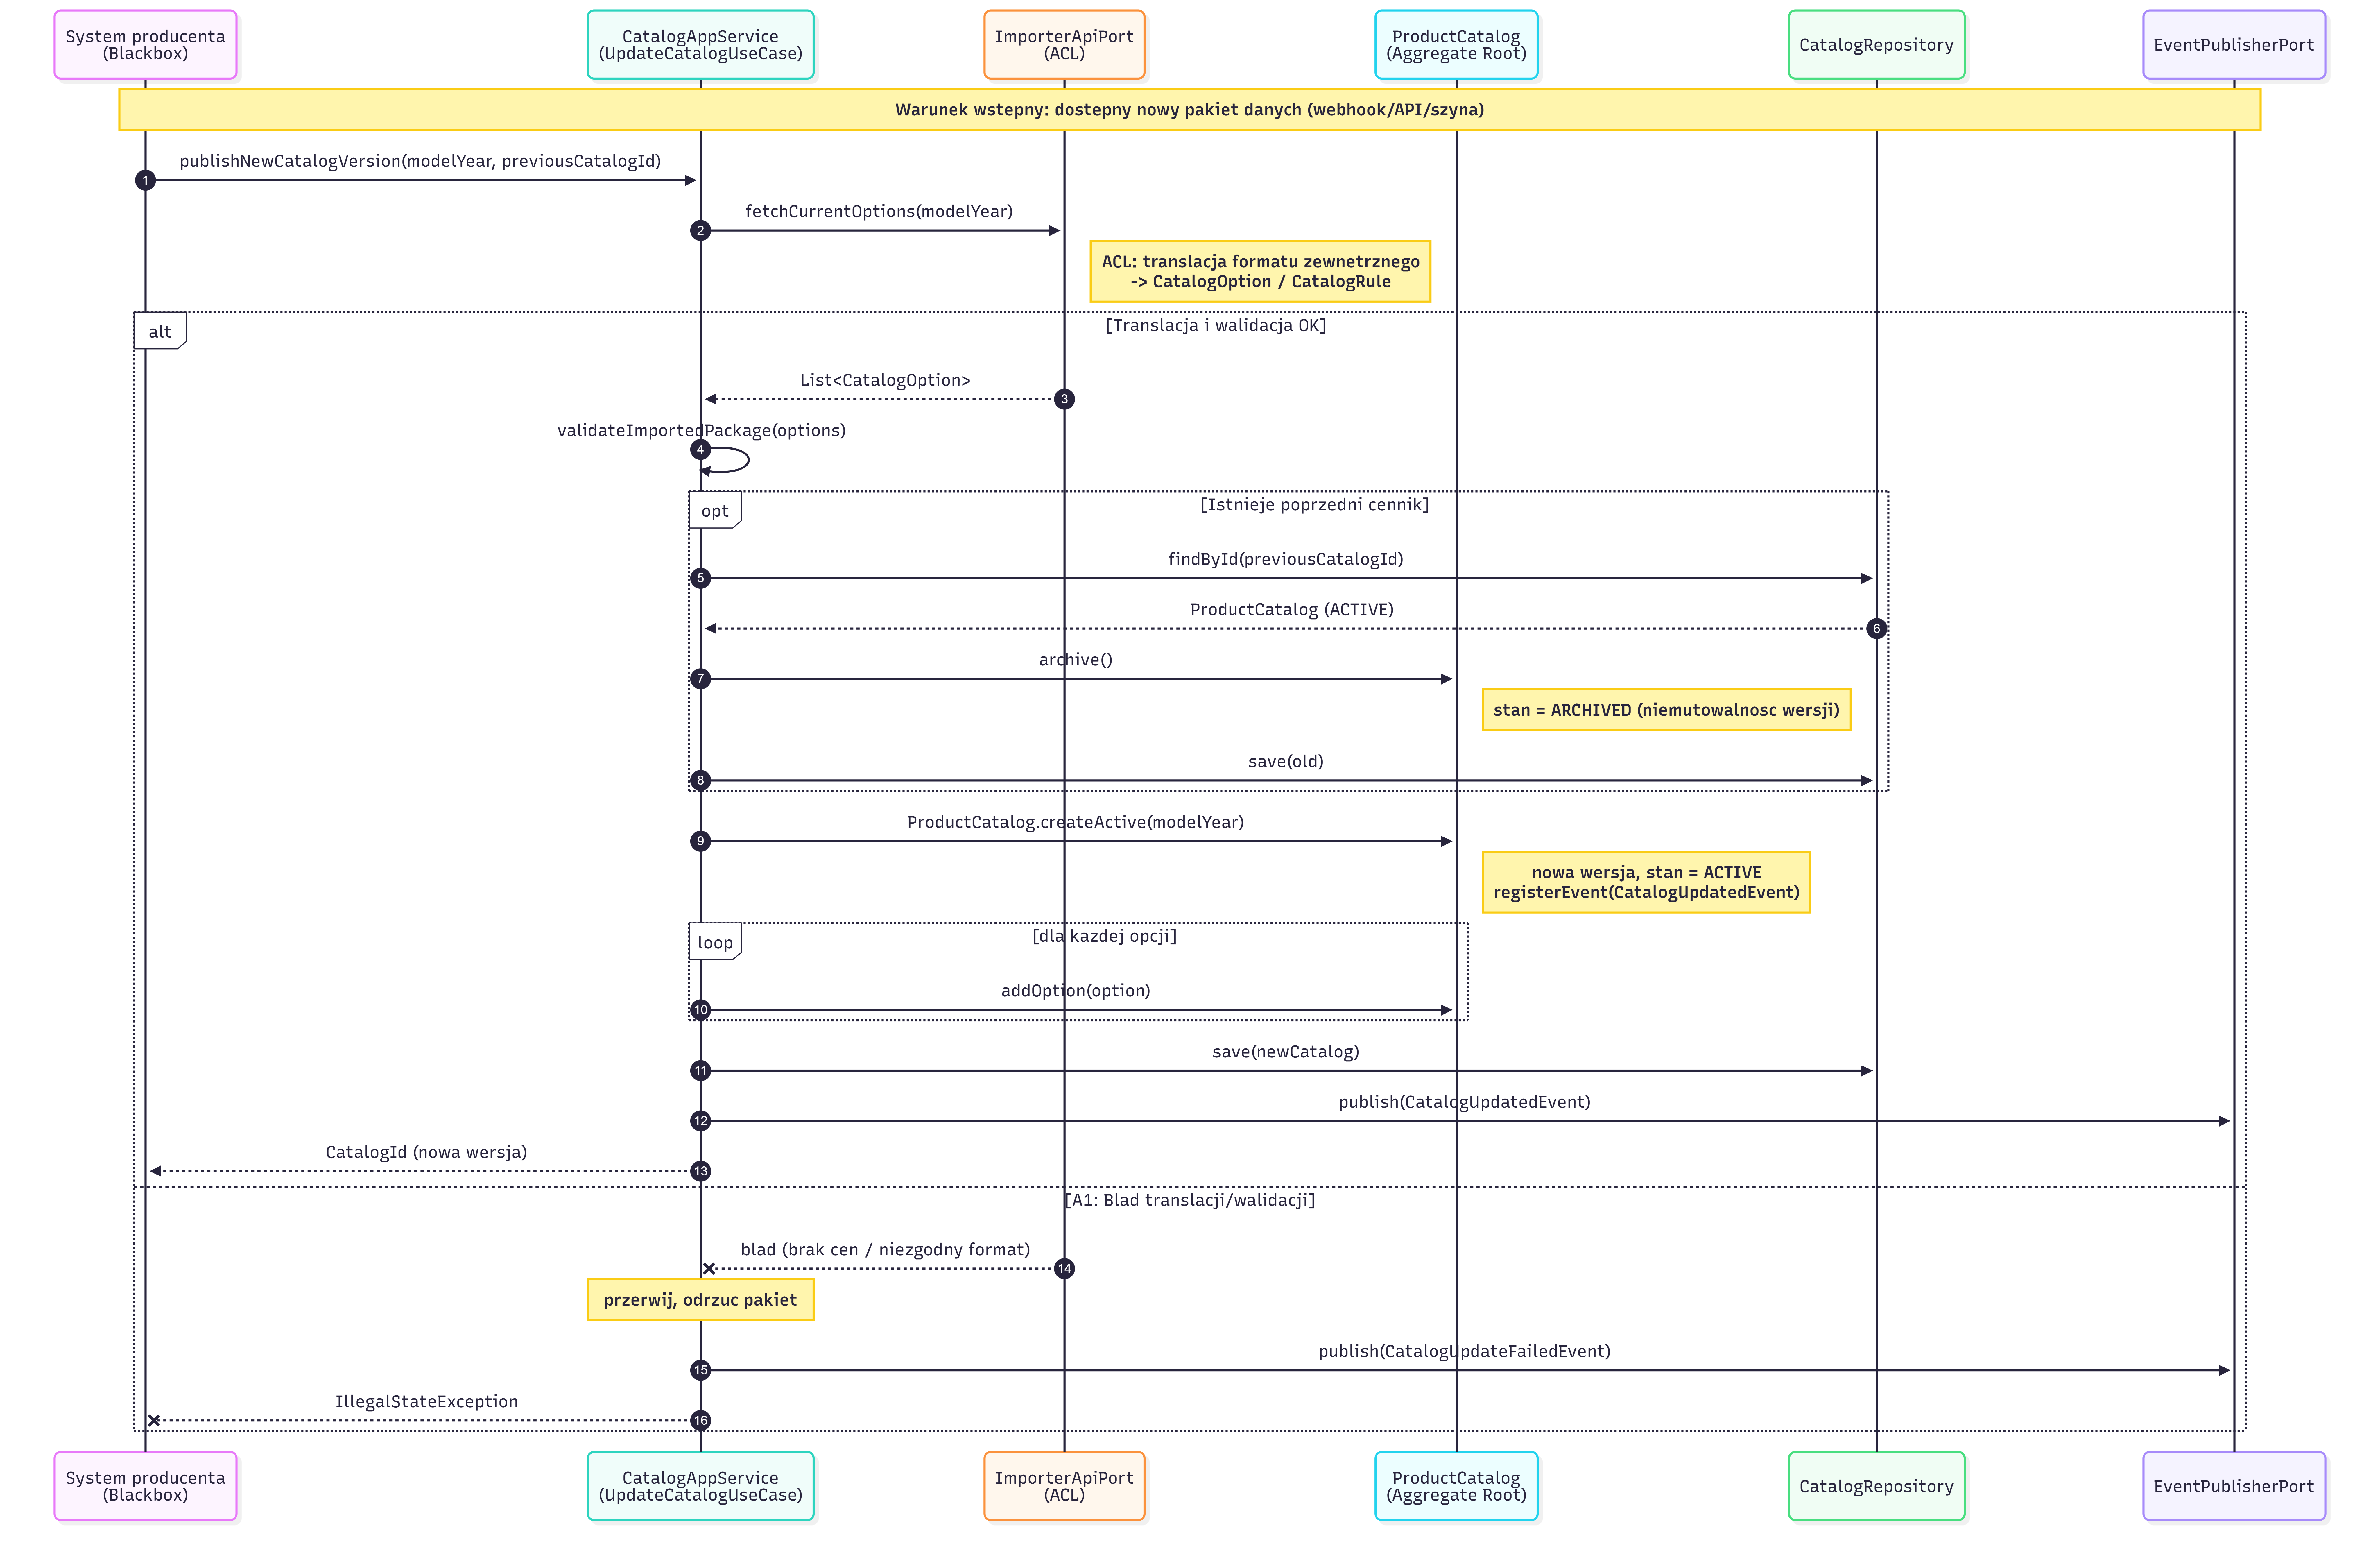
\includegraphics[width=1\textwidth]{media/diagramy_sekwencji/kontekst-katalog/UC-KON-02-Sekwencji.png}
    \caption{Diagram sekwencji dla przypadku użycia UC-KON-02: Automatyczna aktualizacja cennika i katalogu}
    \label{fig:seq_uc_kon_02}
\end{figure}

\subsubsection{Architektura Kontekstu Katalogu i Konfiguratora}

Kontekst Katalogu i Konfiguratora został zaprojektowany w oparciu o architekturę heksagonalną. Diagram Architektury przedstawiono na rysunku \ref{fig:hex_catalog}.

% MIEJSCE NA DIAGRAM ARCHITEKTURY (Katalog Flowchart)
\begin{figure}[H]
    \centering
    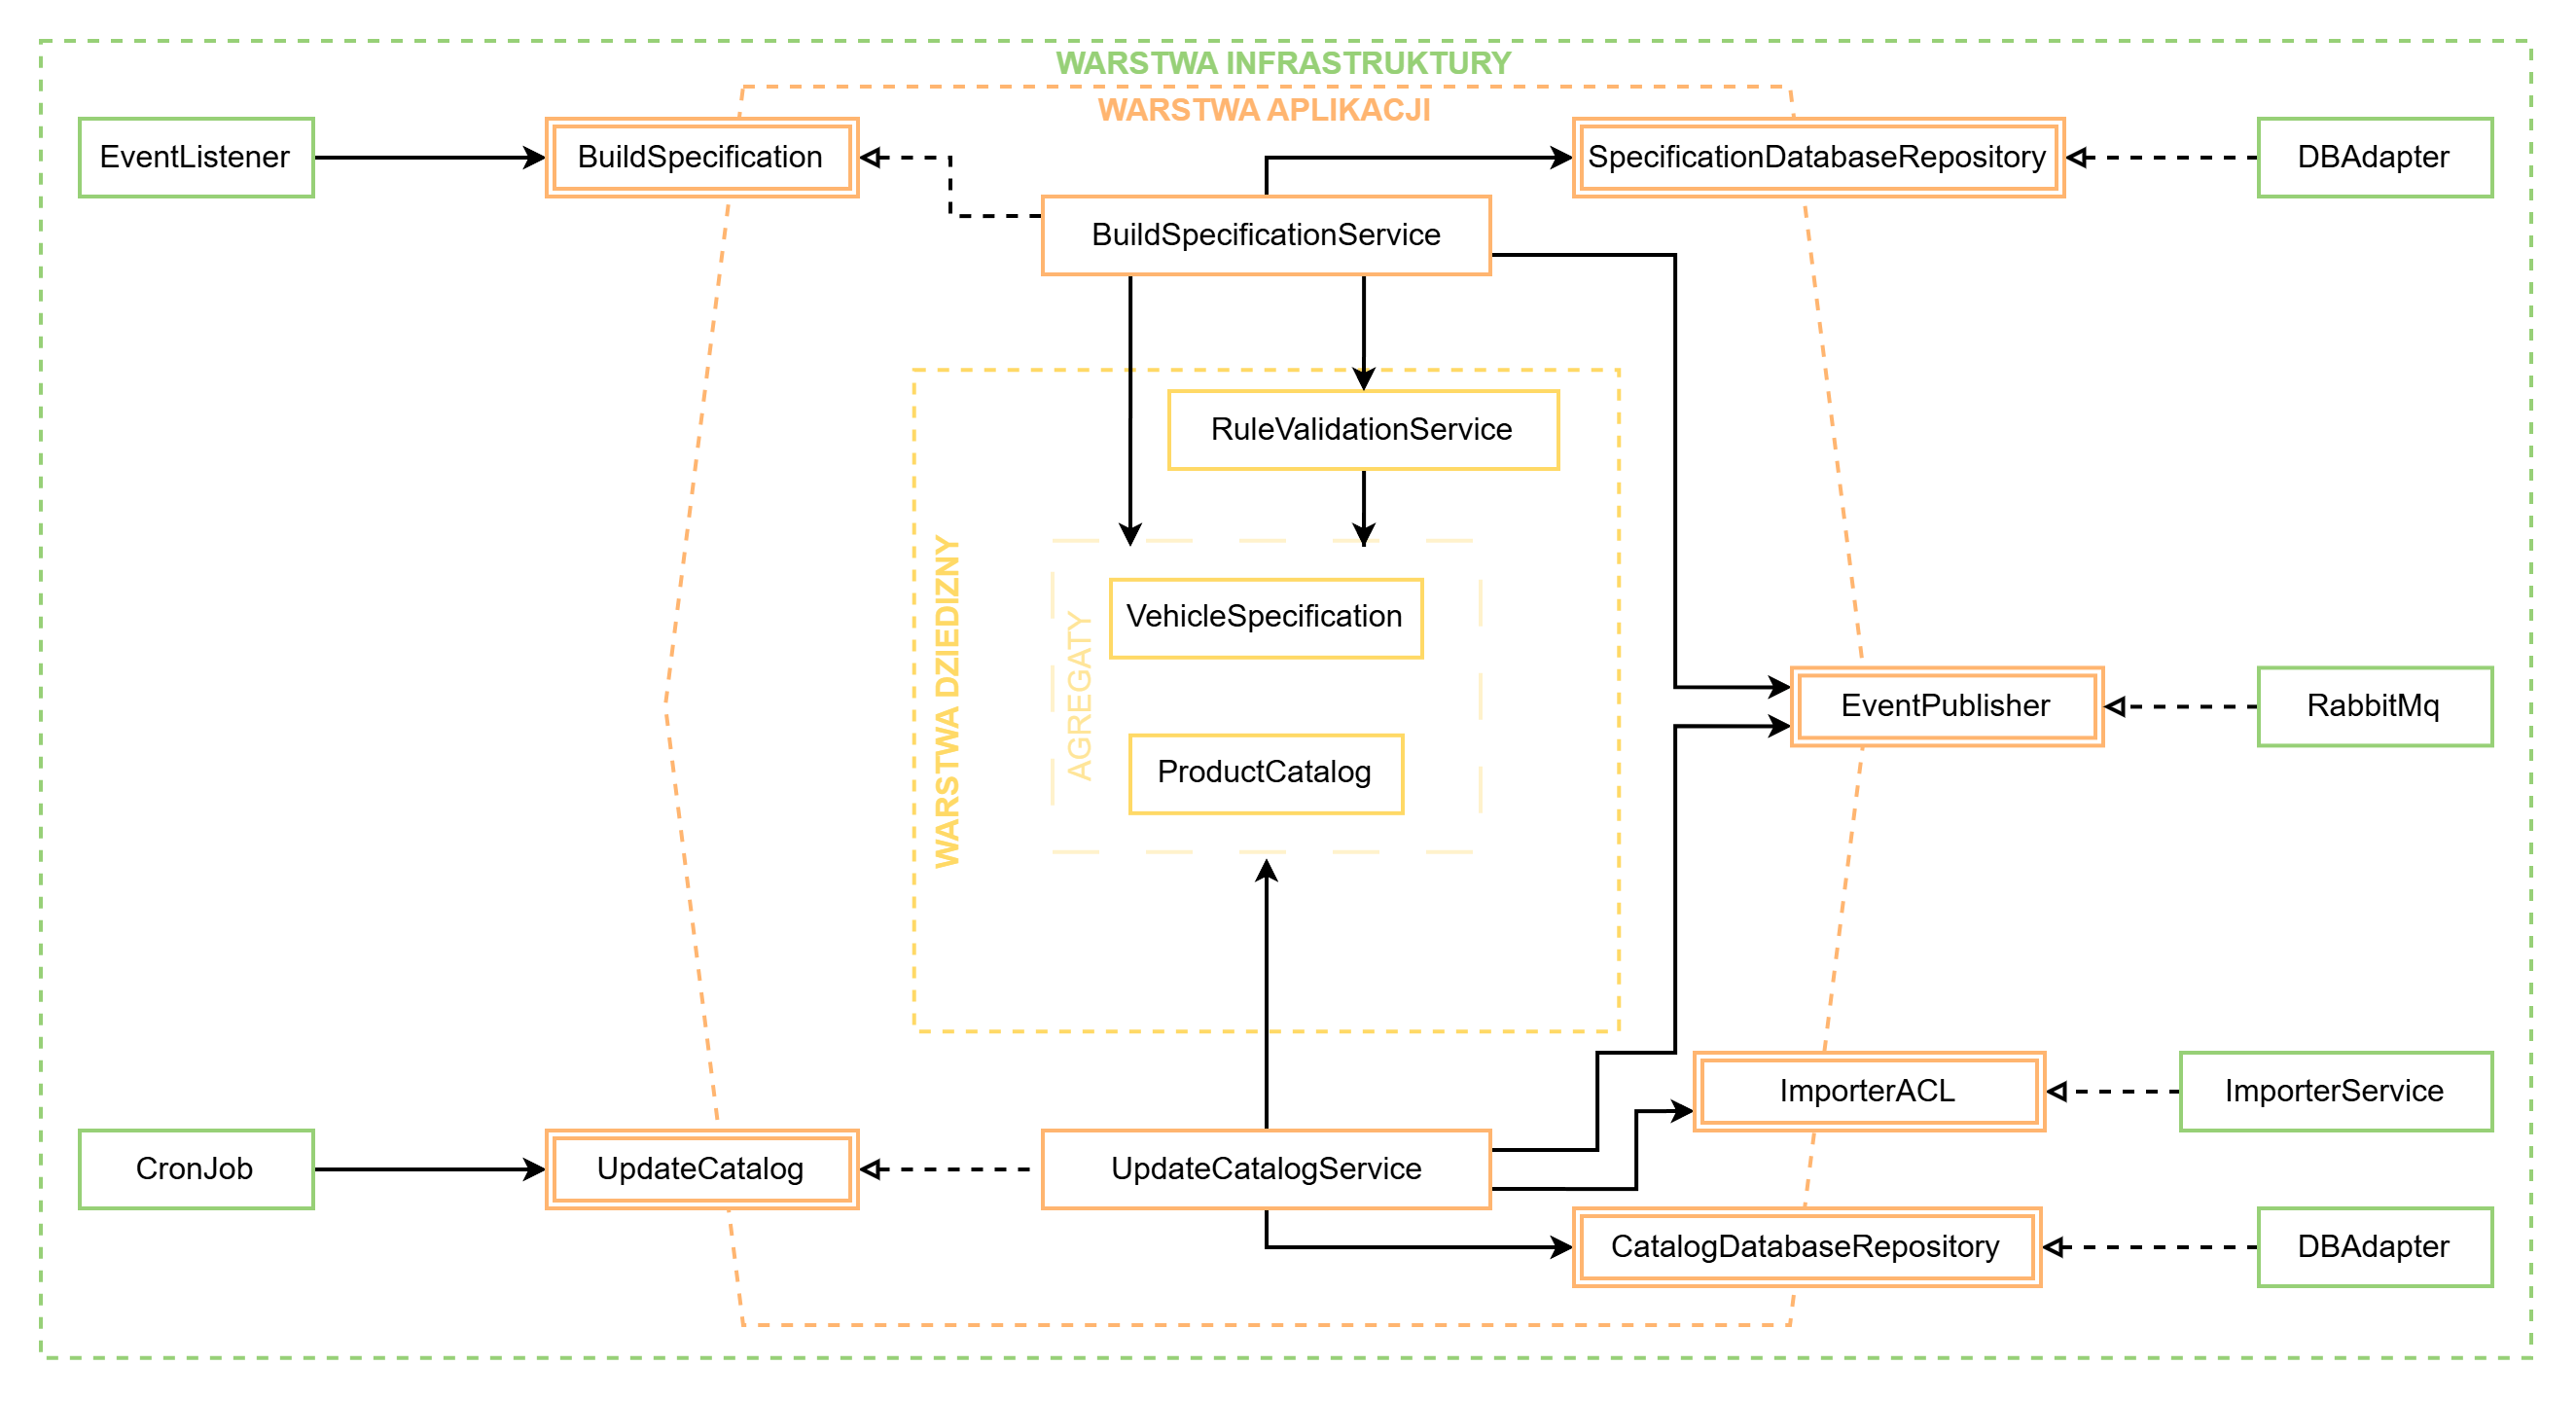
\includegraphics[width=\textwidth]{media/architektura_heksagonalna/CatalogArchitecture.png}
    \caption{Struktura portów i adapterów dla Kontekstu Katalogu i Konfiguratora}
    \label{fig:hex_catalog}
\end{figure}

Poniżej przedstawiono szczegółowy opis interakcji pomiędzy warstwami, z podziałem na strony wejściową i wyjściową.

\paragraph{Strona Wejściowa: Porty i Adaptery} 
Ta strona heksagonu definiuje wejścia do systemu, oddzielając ruch interaktywny od użytkowników od technicznych sygnałów inicjujących aktualizacje.

\begin{itemize}
    \item \textbf{Zarządzanie Specyfikacją Pojazdu (Interaktywne)}
    \begin{itemize}
        \item \textbf{Port:} \texttt{BuildSpecification}. Pojedynczy interfejs obsługujący główny przepływ biznesowy klienta — inicjację (\texttt{startSpecification}), dobór opcji (\texttt{addOption}) i zatwierdzenie (\texttt{finalizeSpecification}) konfiguracji (UC-KON-01). Realizowany centralnie przez \texttt{BuildSpecificationService}.
        \item \textbf{Adapter:} \texttt{ConfiguratorEventListener}. Adapter wejściowy nasłuchujący zdarzeń konfiguratora i tłumaczący je na komendy mutujące stan specyfikacji.
    \end{itemize}

    \item \textbf{Synchronizacja Cennika (Automatyczna)}
    \begin{itemize}
        \item \textbf{Port:} \texttt{UpdateCatalog}. Interfejs inicjujący proces bezpiecznego pobrania i wgrania nowej bazy modelowej (UC-KON-02). Realizowany wyłącznie przez \texttt{UpdateCatalogService}.
        \item \textbf{Adapter:} \texttt{CatalogUpdateScheduler}. Techniczny adapter asynchroniczny wykorzystujący harmonogram zadań, uruchamiający cykliczny proces synchronizacji bazy bez udziału operatora.
    \end{itemize}
\end{itemize}

\paragraph{Strona Wyjściowa: Porty i Adaptery} 
Ta strona heksagonu zarządza utrwalaniem zwalidowanych danych we własnej bazie oraz wymianą danych z globalnym systemem producenta.

\begin{itemize}
    \item \textbf{Integracja z Producentem (Warstwa Ochronna)}
    \begin{itemize}
        \item \textbf{Port:} \texttt{CatalogImporterPort}. Interfejs służący do pobierania zewnętrznych danych o regułach, opcjach i cenach.
        \item \textbf{Adapter:} \texttt{ImporterAclAdapter} (wraz z \texttt{ImporterServiceClient}, \texttt{ImporterCatalogTranslator}, \texttt{ExternalCatalogPackage}). Implementuje wzorzec Anti-Corruption Layer — tłumaczy zagnieżdżone, potencjalnie niestabilne struktury API dostawcy na czysty, wewnętrzny model obiektów wartości, izolując rdzeń katalogu od zmian formatu u importera.
    \end{itemize}

    \item \textbf{Utrwalanie Stanu (Persystencja)}
    \begin{itemize}
        \item \textbf{Porty:} \texttt{VehicleSpecificationRepository} oraz \texttt{ProductCatalogRepository}. Umożliwiają trwały zapis odpowiednio konfigurowanych specyfikacji aut oraz wersjonowanych wydań katalogów.
        \item \textbf{Adaptery:} \texttt{SpecificationDatabaseRepository} oraz \texttt{CatalogDatabaseRepository} (z mapperami \texttt{*PersistenceMapper} i rekordami \texttt{*Record} oraz \texttt{DbAdapter}/\texttt{InMemoryDbAdapter}). Mapują grafy obiektów domenowych na rekordy magazynu, gwarantując zapis z zachowaniem spójności; w bieżącej implementacji warstwą bazową jest \texttt{InMemoryDbAdapter}.
    \end{itemize}

    \item \textbf{Publikacja Zdarzeń (Event Driven)}
    \begin{itemize}
        \item \textbf{Port:} \texttt{EventPublisher}. Umożliwia publikację zdarzeń wynikowych na magistralę.
        \item \textbf{Adapter:} \texttt{RabbitMqEventPublisher} (wraz z \texttt{MessageBroker}). Serializuje zdarzenia dziedzinowe (np. \texttt{SpecificationCompleted}, \texttt{CatalogUpdated}) i wysyła je na magistralę.
    \end{itemize}
\end{itemize}

\paragraph{Usługi Aplikacji}
Ze względu na konieczność separacji procesu tworzenia cennika od procesu jego konsumpcji, wyodrębniono tu dwa niezależne orkiestratory:
\begin{itemize}
    \item \textbf{BuildSpecificationService} – zarządza cyklem życia agregatu \texttt{VehicleSpecification}. Przechwytuje żądania użytkownika, deleguje rygorystyczną weryfikację reguł wykluczających do serwisu domenowego, a po ostatecznym zatwierdzeniu utrwala specyfikację i emituje fakt o ukończeniu konfiguracji (\texttt{SpecificationCompleted}).
    \item \textbf{UpdateCatalogService} – orkiestruje proces zapisu cennika. Zamiast nadpisywać istniejące dane, tworzy nową instancję agregatu \texttt{ProductCatalog} z podbitą wersją, oznaczając stary katalog jako archiwalny, co chroni integralność historycznych zamówień, i emituje \texttt{CatalogUpdated}.
\end{itemize}

\paragraph{Usługi Domenowe}
Ze względu na złożoność wykluczeń inżynieryjnych (np. niekompatybilność danego silnika z konkretną skrzynią biegów), wdrożono dedykowany serwis bezstanowy:
\begin{itemize}
    \item \textbf{RuleValidationService} – izoluje skomplikowaną logikę weryfikacyjną. Zgodnie z zasadami projektowania domenowego agregat specyfikacji nie posiada wiedzy o zewnętrznym cenniku — to serwis aplikacyjny deleguje walidację do tego serwisu domenowego, który (sam pobierając katalog z repozytorium) ocenia legalność wybranych kombinacji kodów opcji przed przejściem do stanu końcowego.
\end{itemize}

\subsubsection{Agregaty Kontekstu Katalogu i Konfiguratora}

Aby zapewnić odporność systemu na zmianę cen w trakcie długotrwałego procesu ofertowania, zastosowano twardy rozdział pomiędzy słownikiem reguł a koszykiem konfiguracyjnym użytkownika, tworząc dwa oddzielne agregaty.

% MIEJSCE NA DIAGRAM KLAS: ProductCatalog
\begin{figure}[H]
    \centering
    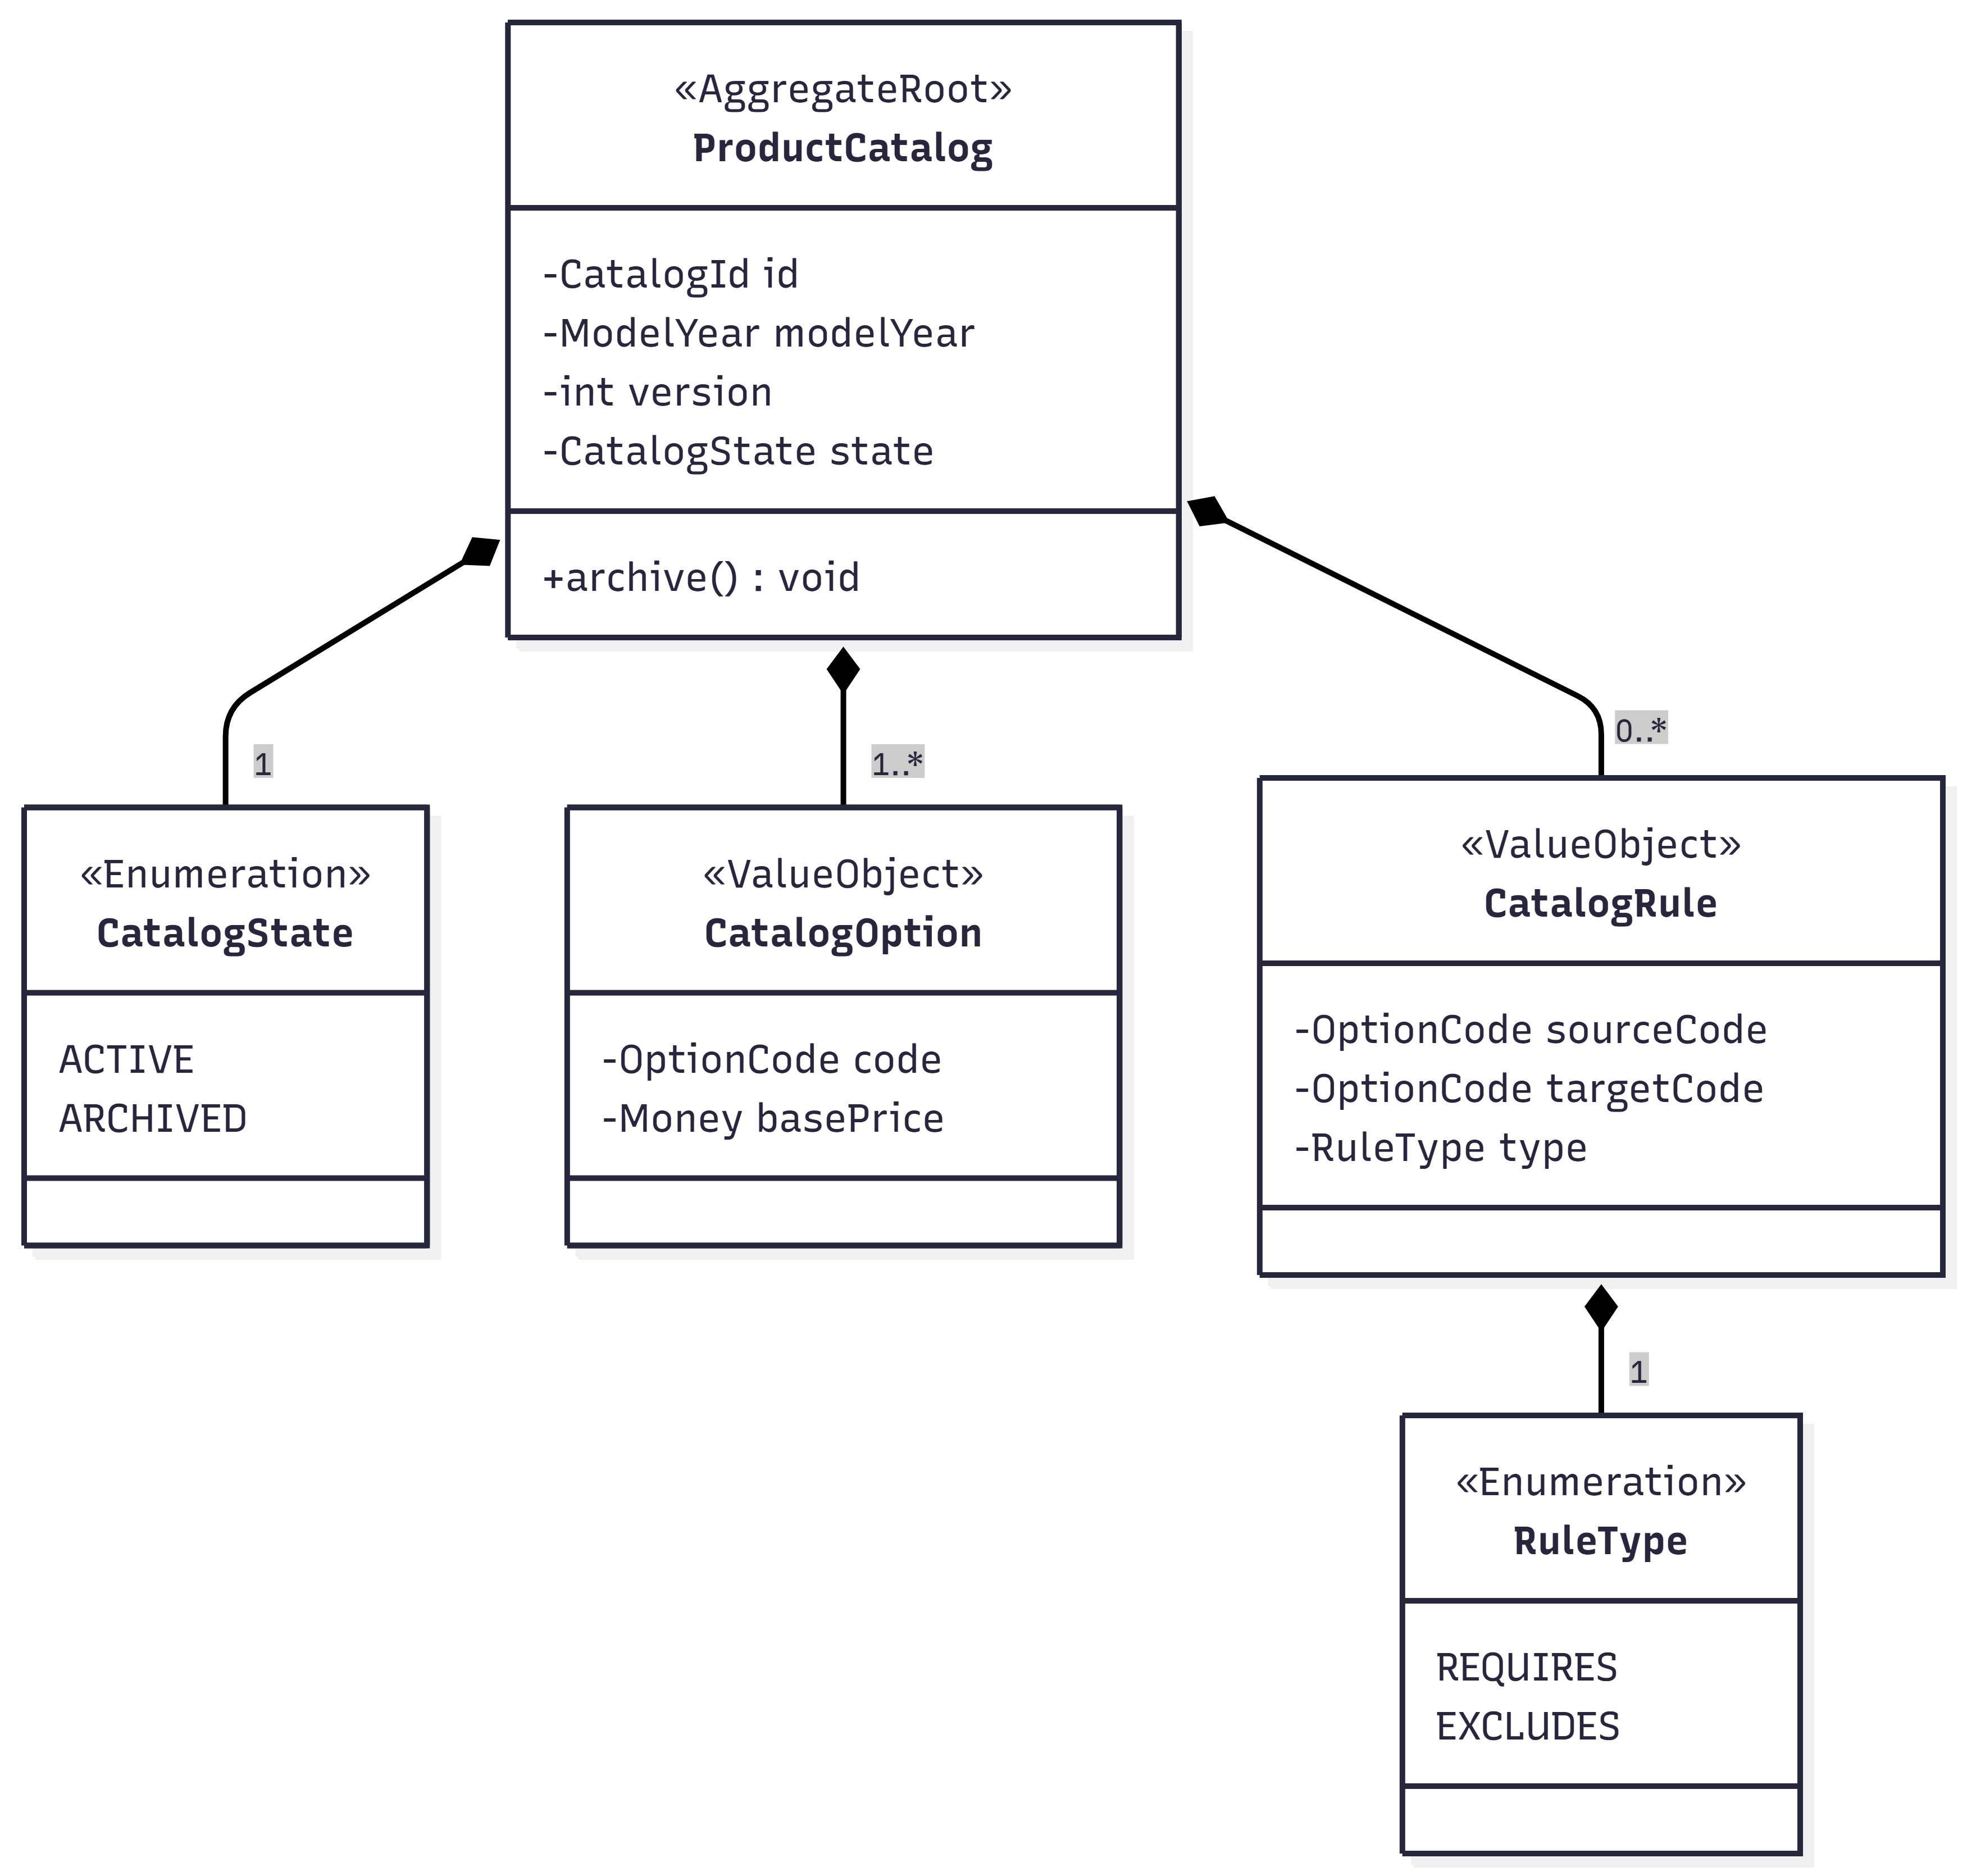
\includegraphics[width=0.49\textwidth]{media/agregaty/kontekst-katalogu/product-catalog.png}
    \hfill
    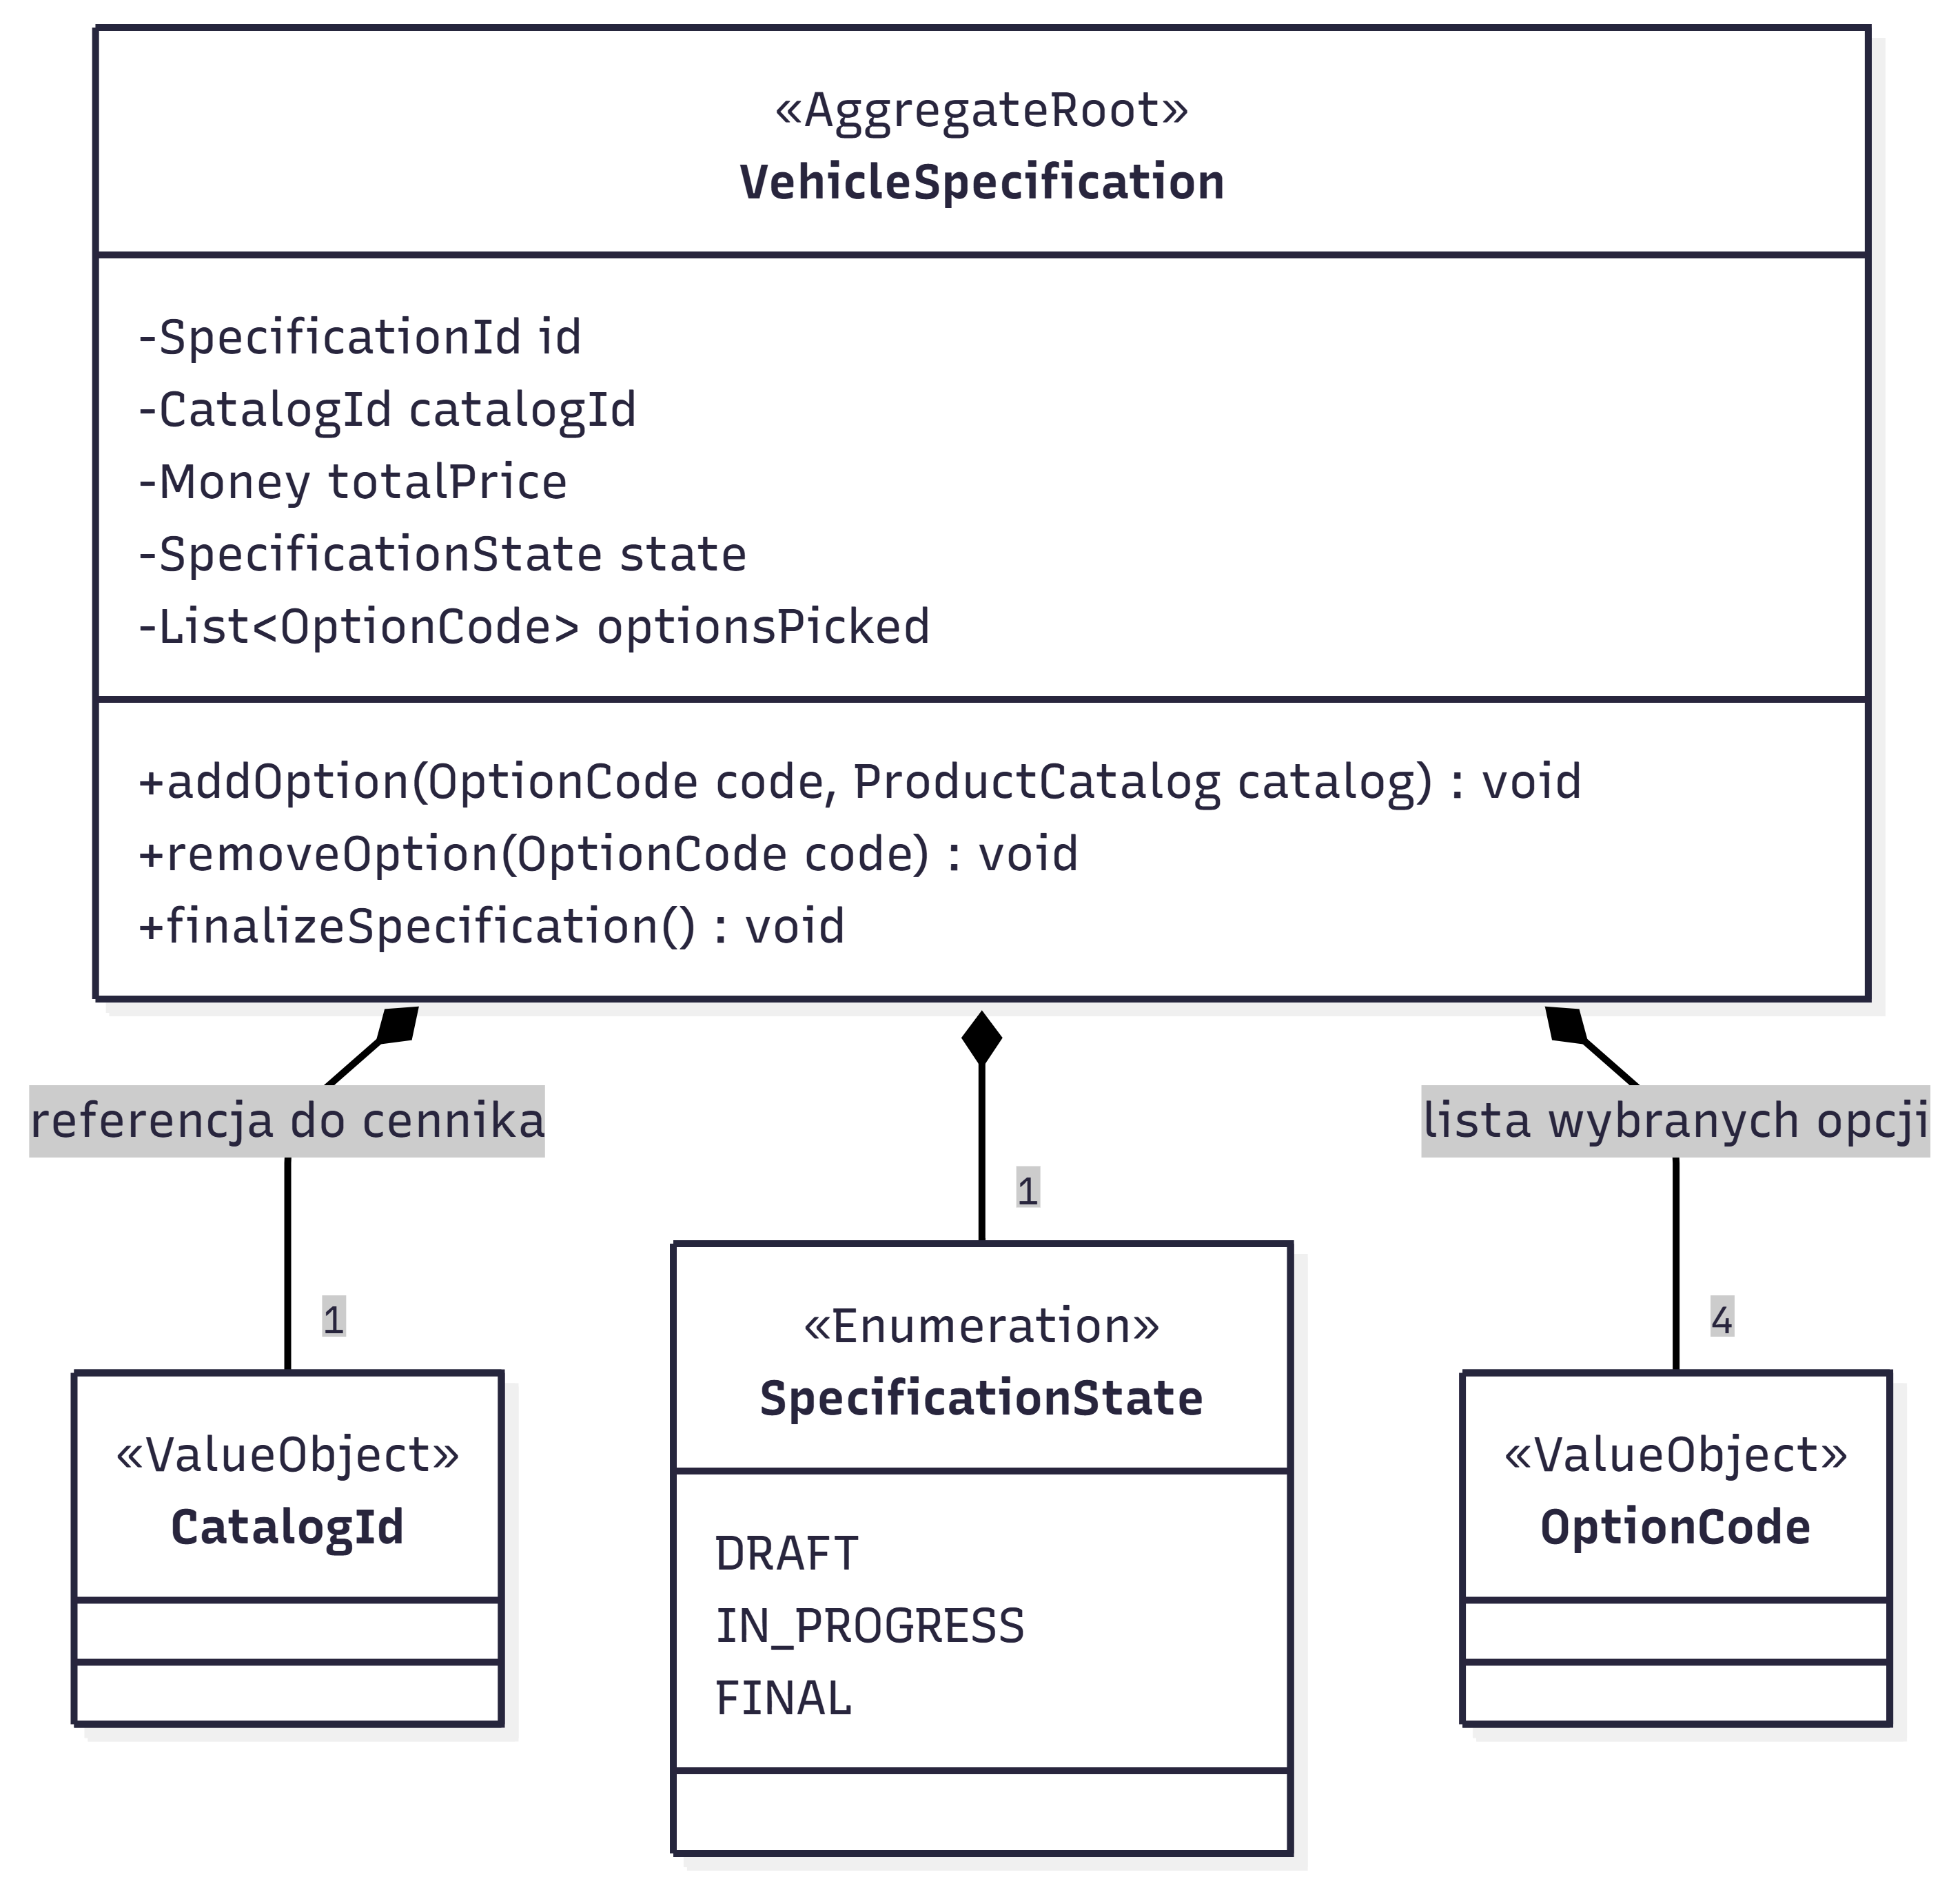
\includegraphics[width=0.49\textwidth]{media/agregaty/kontekst-katalogu/vehicle-spec.png}
    \caption{Model strukturalny agregatu Matrycy Produkcyjnej}
    \label{fig:agg_product_catalog}
\end{figure}

\paragraph{Agregat: Matryca Produkcyjna / Cennik (ProductCatalog)}
Agregat ten stanowi kompletny zbiór opcji (\texttt{CatalogOption}) i reguł zależności (\texttt{CatalogRule}) przypisany do danego rocznika modelowego.
\begin{itemize}
    \item \textbf{Ochrona Niezmienników (Niemutowalność wersji):} Cennik będący w stanie \texttt{ACTIVE} jest obiektem ściśle niemutowalnym. Jakakolwiek aktualizacja cen lub reguł pobrana z API producenta nie może nadpisać aktywnego obiektu -- wzorzec fabryki wymusza stworzenie nowej wersji (\texttt{version}) agregatu i dearchiwizację starej. Gwarantuje to, że historyczne specyfikacje klientów zachowują bezwzględną spójność z cennikiem, z którego zostały wygenerowane.
    \item \textbf{Polityka pakietowa:} Zgodnie z założeniami biznesowymi, słownik \texttt{OptionCode} nie operuje na pojedynczych elementach (tzw. mikrozarządzanie wyposażeniem), lecz na bazie predefiniowanych zbiorów (np. Wersja Wyposażenia, Silnik, Skrzynia Biegów, Kolor). Znacznie optymalizuje to wydajność mechanizmów walidacyjnych w systemie.
\end{itemize}

\paragraph{Agregat: Specyfikacja Pojazdu (VehicleSpecification)}
Reprezentuje unikalną konfigurację budowaną przez klienta lub handlowca, identyfikowaną przez globalny unikalny numer \texttt{SpecificationId}.
\begin{itemize}
    \item \textbf{Maszyna Stanów i Kompletność (\texttt{IN\_PROGRESS}):} Specyfikacja podlega ścisłemu cyklowi stanowemu. Początkowo tworzona jest jako pusty \texttt{DRAFT}. Gdy użytkownik rozpoczyna wybór opcji, agregat przechodzi w stan \texttt{IN\_PROGRESS}. Stan ten oznacza, że konfiguracja jest w toku budowy i nie posiada jeszcze kompletu wymaganych do produkcji makro-opcji (np. brakuje wyboru docelowego silnika, skrzyni biegów czy koloru).
    \item \textbf{Ochrona Niezmienników (Walidacja Technologiczna):} Próba dodania nowej opcji wyposażenia (metoda \texttt{addOption}) na bieżąco weryfikuje lokalną listę wybranych kodów względem reguł (\texttt{EXCLUDES}, \texttt{REQUIRES}) dostarczonych przez serwis domenowy na podstawie cennika. Złamanie reguły natychmiastowo blokuje operację (wzo